\documentclass{article}
\usepackage{pgfplots}
\usepackage{multirow}
\usepackage{rotating}
\usepackage[]{float} 
\usepackage{hyperref} 
\usepackage[a4paper, total={6in, 8in}]{geometry}
\usepackage{booktabs}
\usepackage{subcaption}
\usepackage{amsfonts}
\title{The Bubble Algorithm Library}
\author{Experiment 2, Experimentation \& Evaluation, 2022\\Arnaud Fauconnet,
	Francesco Costa}
\date{}

\usepackage[most]{tcolorbox}


\newtcbtheorem{Hypotheses}{\bfseries Hypotheses}{enhanced,drop shadow={black!50!white},
	coltitle=white,
	top=0.3in,
	attach boxed title to top left=
		{xshift=1.5em,yshift=-\tcboxedtitleheight/2},
	boxed title style={size=small,colback=black}
}{summary}


\begin{document}
\maketitle
\tableofcontents

\section*{Abstract}
Reading text can be difficult, especially in an informatics setting in which variable names have to be clear, meaningful and 
easy to understand. The aim of this experiment is to find whether the use of specific separators when writing composed identifiers 
can, just as for natural language, lead to substantial reading speedups. The chosen separation methods are the commonly used camelCase and 
kebab-case. In general the choice of a particular writing practice comes down to personal preference, but we now want to study these two 
specific options to see if we can objectively deem one better than the other. The experiment is run by asking users to select a short phrase (two or three words) 
created using one the two separation methods among four possible options, with the objective of finding the one corresponding to an example phrase 
separated by spaces.

\newpage 
\section{Introduction}
The experiment focuses on text readability and specifically reading phrases creted using different separators. Programmers usually decide on the formatting of 
variable names based on either personal preference or feelings on the day. Our objective is to find out if there is an objectively superior separator, which would 
not only improve the experience of the individual programmer but also standardize naming conventions in team settings, leading to a more 
efficient group working environment.
We know from prior research that the use of any separator in natural language leads to significant increases in reading speed. The question is whether this translates in 
code and if there is a superior separator. 

To find the desired results we have designed an experiment for users to partake in which is meant to show the difference in using two specific separators commonly 
used in informatics: camelCase and kebab-case. The users will be presented with a phrase (composed by two or three words) separated by spaces and will be asked to choose between four options 
written using one of the two separators the one corresponding to the original phrase. The performance of the user will be measured by taking into account the time needed to 
find the correct solution and the actual result of whether they chose correctly or not.


\begin{Hypotheses*}{Most effective separator}{}
	Given that prior research simply proved an increase in performance when using any separator, and the fact that 
	programmers usually have a preferred formatting for variables, we don't expect camelCase or kebab-case to perform 
	significantly better than the other.
\end{Hypotheses*}

\section{Method}
\subsection{Variables}
The chosen separators will be used as variables when running the experiment. The age of the participant as well as their proficiency in programming 
will also be set at the start of each experiment
\begin{description}
	\item[Separator] we want to see whether the use of a specific formatting will lead to any improvement in reading speed and text comprehension. 
	The two separators chosen are simply among the most commonly used when writing code and approach the problem of 
	splitting text in different ways
	\begin{description}
		\item[camelCase] this is the first separator, which makes use of capital letters to distinguish between words;
		\item[kebab-case] the second separator relies instead on a special character (-) to split a phrase in different words.
	\end{description}
	\item[Age] we expect that age would lead to significant differences in performance, regardless of separation method;
	\item[Programming background] we expect programmers to already be used to the separators used, hence resulting in better results when considering 
	similar or same age.
\end{description}

The dependent variables are the time taken to complete each task (in milliseconds) and the correctness of the results (boolean value). By using and combining these 
two measures we hope to be able to see perceivable differences (or the absensce of them) in order to compare the two separators.

For control variables we have decided to let every user run the experiment on our machine (which will be specified in the apparatus section) using 
the build in trackpad. We have also tried to run the experiment during the same time slots (afternoon from 14 to 18) hoping that this would 
bring some consistency in the physiological state of the user (not too tired or just woken up).

\subsection{Design}
The experiment is designed with fixed tasks that lead to precise results in order to cotrol the environment as much as possible. The uncertainty that 
user bring to experiment is controlled by having tasks that give us measures that can directly be used in order to analyse results. The set of users asked to 
perform the experiment are not divided between the different separators, meaning all users perform tasks related to both formatting methods. This resembles the 
within subject design expect the experiment is only run once per user by asking question regarding camelCase and kebab-case in a random order. This is to prevent 
the test subject to be able to predict which separator will be used in the next task, hence making it impossible for her/him to "prepare".

\subsection{Participants}
The participants of the experiment were chosen mainly among the students of the faculty of informatics at USI. We did manage to get at least some user 
with different backgrounds and ages, but most of the results will be from subject with programming knowledge and an age between 20 and 25. Since we are testing the difference 
between two separators there is no control group and all participants were asked the same questions, half usings camelCase, half using kebab-case.

\subsection{Apparatus and Materials}
We run all tests on the same machine, the specs are as follows:
\label{apparatus}
\begin{center}
	\begin{tabular}{ll}
		\hline
		\hline
		\textbf{Computer Model} &  Lenovo Thinkpad X1 Carbon\\
		\hline
		\textbf{Processor}      &  i7 8550u (8 cores)\\
		\textbf{Graphics Card}  &  UHD Graphics 620\\
		\textbf{Memory}         &  16GB \\
		\textbf{OS}             &  Arch Linux\\
		\hline
		\hline
	\end{tabular}
\end{center}

\subsection{Procedure}
The procedure of running an experiment consisted simply in asking a participant to complete tasks on a site run locally on our machine. 
The user were met with a welcome page introducing the general idea of the project followed by a form used to gather information such as the 
name of the participant, her/his age and their proficiency in programming. Finally, before getting into the actual testing phase, an example 
task was shown in order to properly explain what to expect and to let the user get accustomed to the interface. The actual tasks consisted in 
22 short phrases (two or three word long) for which the objective was to find a matching entry among the possible choices written using a 
specific formatting method (half in camelCase, half in kebab-case).
Each experiment took around 2/3 minutes.
\section{Results}

\subsection{Visual Overview}
By plotting the distribution of average times taken for camelCase and kebab-case we can get a first visual comparison of the two. 
From the following graphs we can see that the distribution of times for kebab-case is heavily shifted towards the shorter time averages, while 
for camelCase it is much more spread.

\begin{figure}[h!]
    \centering
		\begin{subfigure}{0.49\textwidth}
			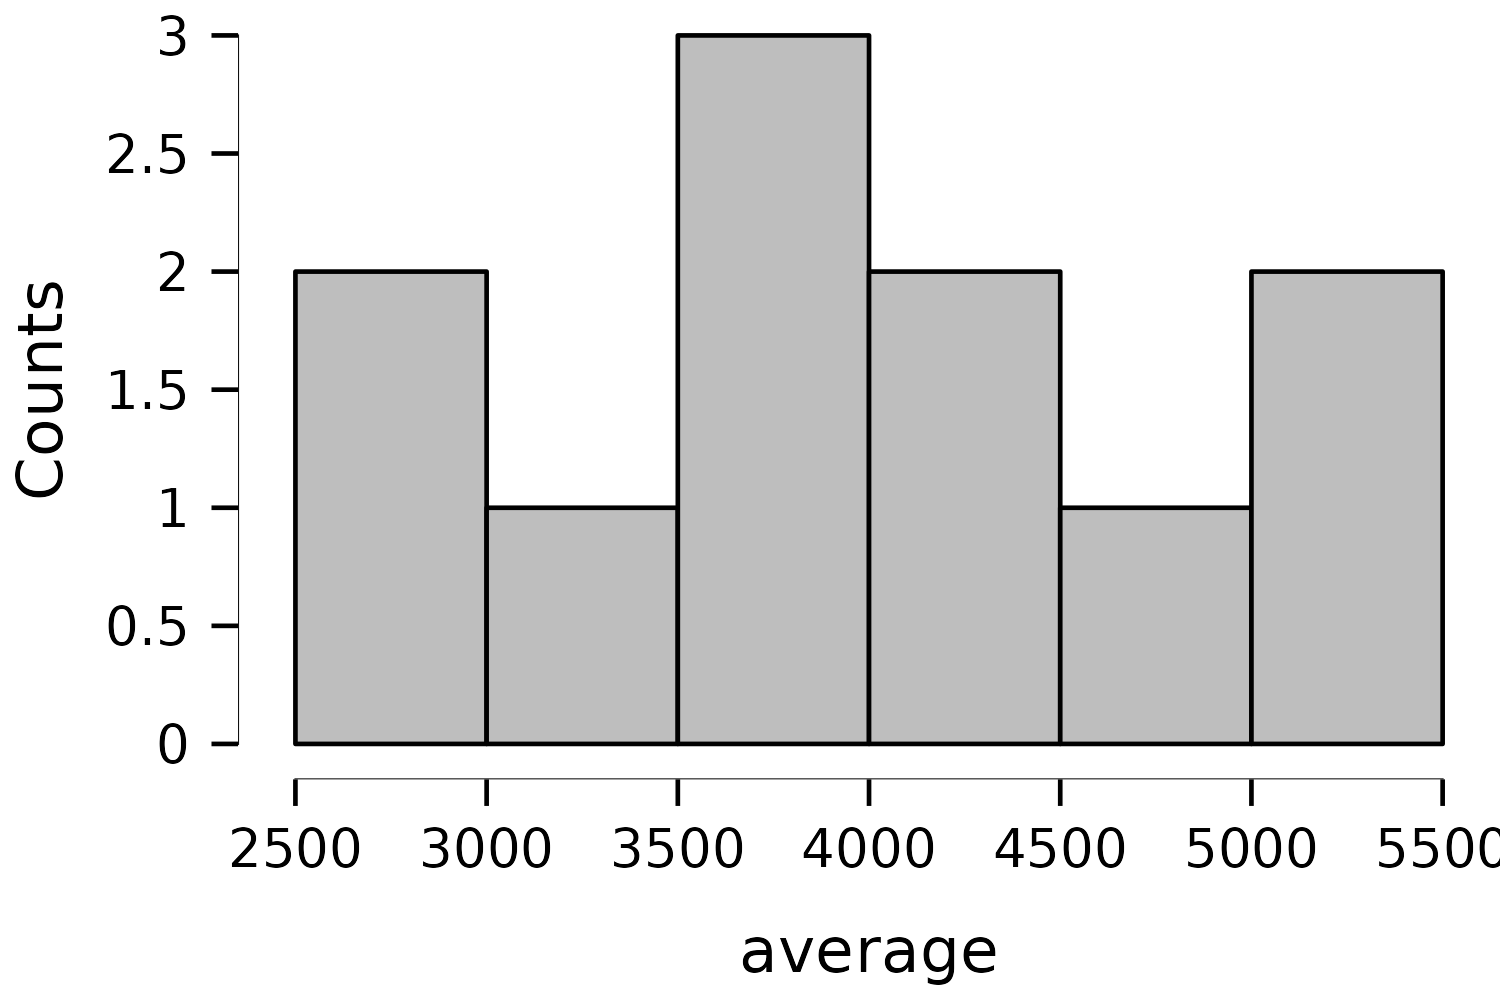
\includegraphics[width=\textwidth]{images/avg_camel.png}
			\caption{Distribution of average time for camelCase}
		\end{subfigure}
		\begin{subfigure}{0.49\textwidth}
			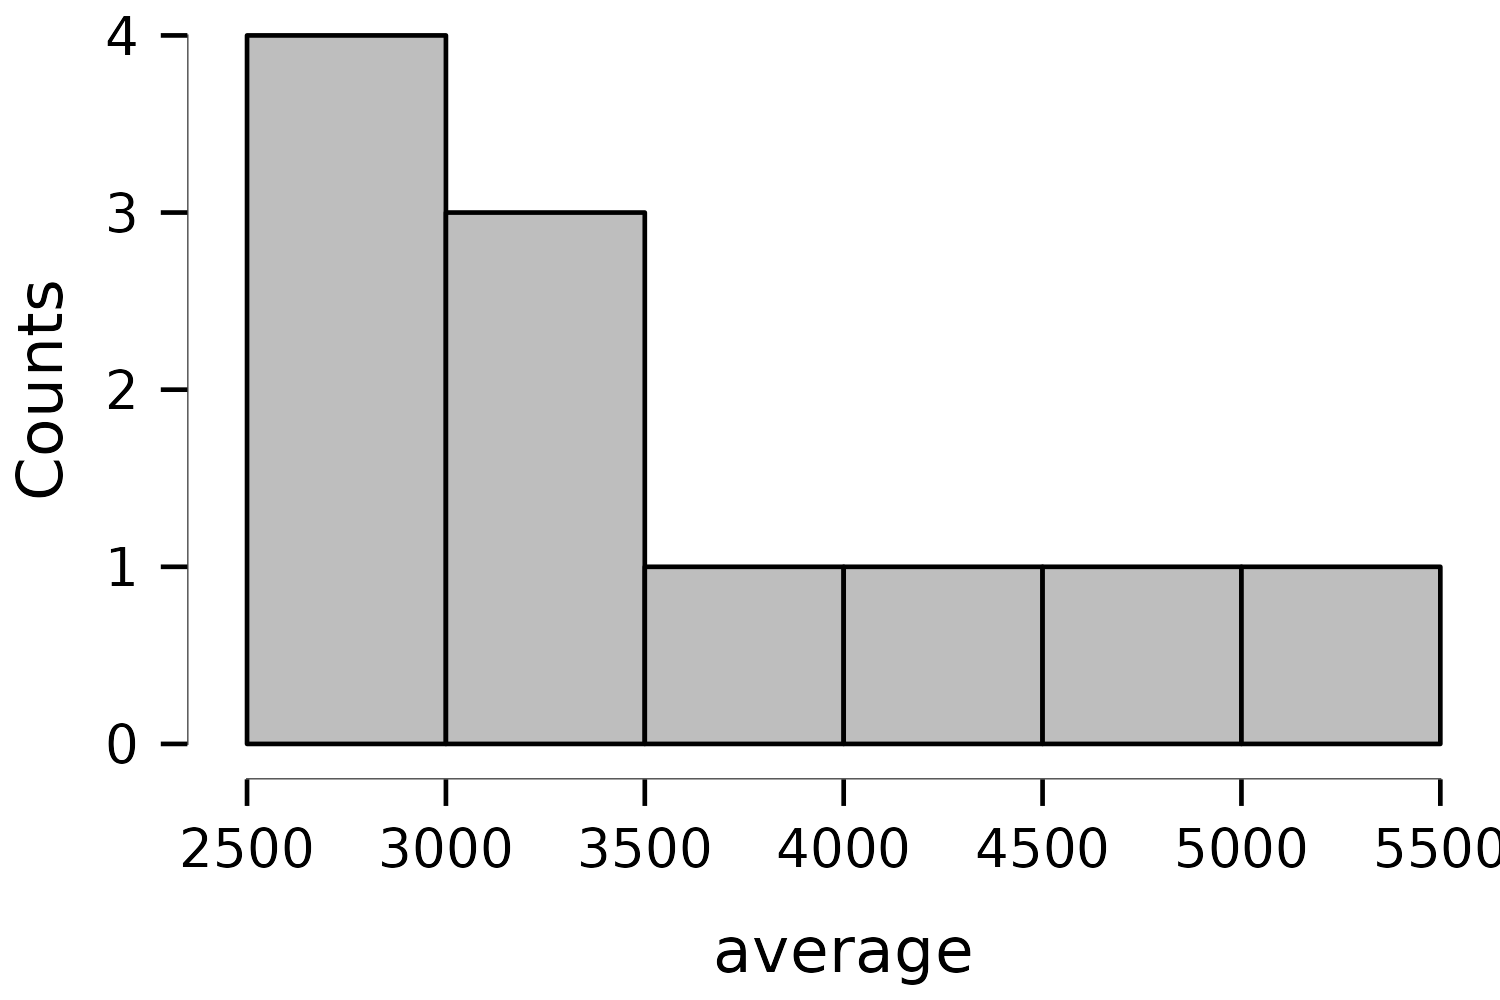
\includegraphics[width=\textwidth]{images/avg_kebab.png}
			\caption{Distribution of average time for kebab-case}
		\end{subfigure}
\end{figure}

This makes us think that in general participants had a better performance using kebab-case and we can also see it when 
looking at the average time taken depending on the length of the phrase. It is pretty clear that the curve that interpolates the points of the graphs 
is significantly lower for kebab-case.

\begin{figure}[h!]
    \centering
		\begin{subfigure}{0.49\textwidth}
			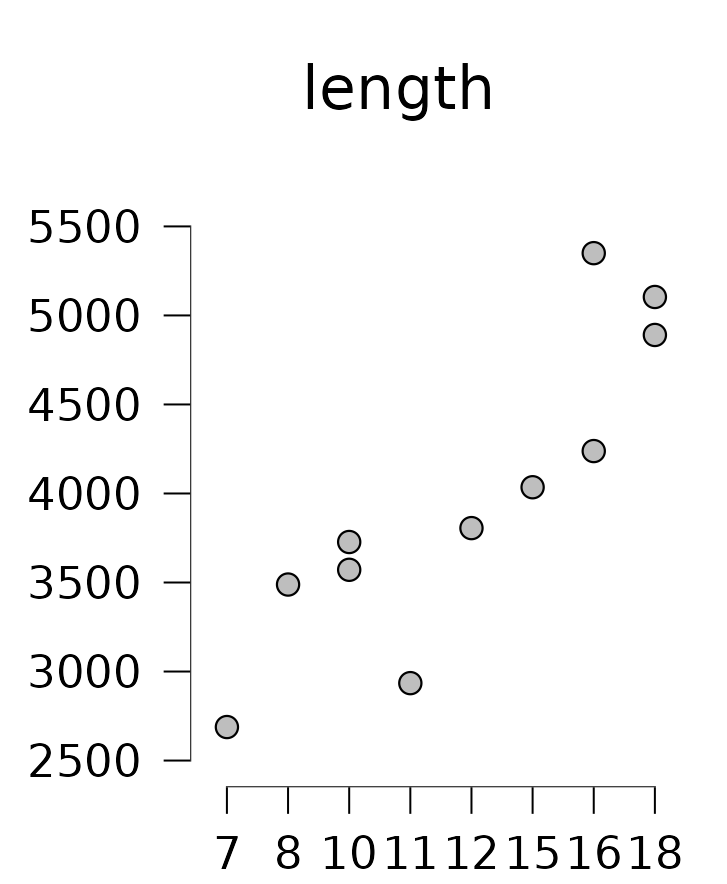
\includegraphics[width=.8\textwidth]{images/time_length_camel.png}
			\caption{Average time depending on length of phrase for camelCase}
		\end{subfigure}
		\begin{subfigure}{0.49\textwidth}
			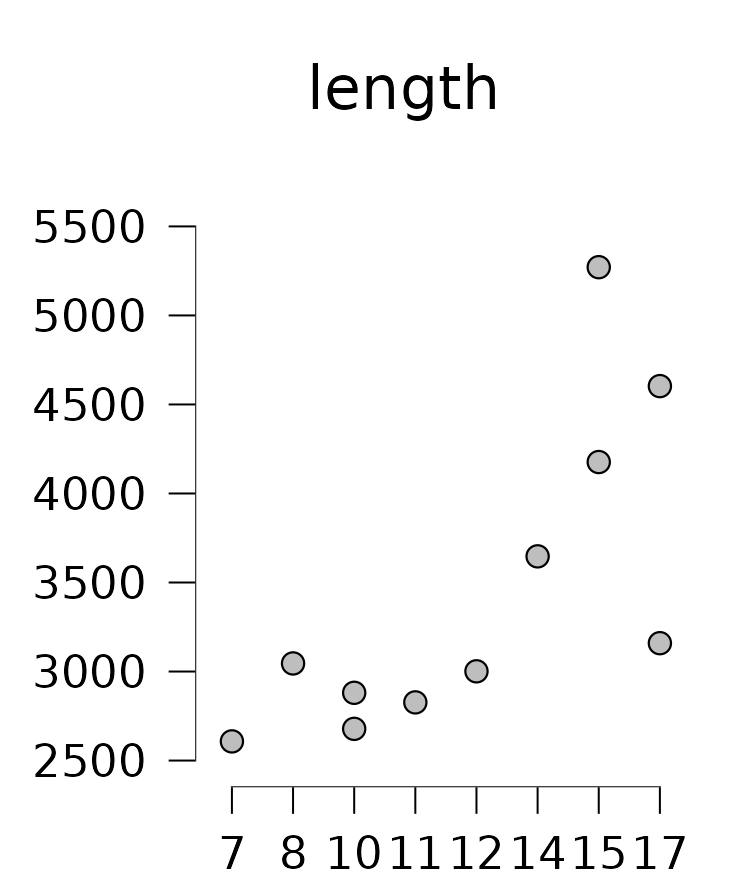
\includegraphics[width=.8\textwidth]{images/time_length_kebab.png}
			\caption{Average time depending on length of phrase for kebab-case}
		\end{subfigure}
\end{figure}

Looking at the relation between average time and proficiency in programming we can clearly see from the following graph that participants with 
prior programming knowledge managed to complete the tasks with a lower distribution of average times compared to those without coding experience.

\begin{figure}[h!]
    \centering
		\begin{subfigure}{0.49\textwidth}
			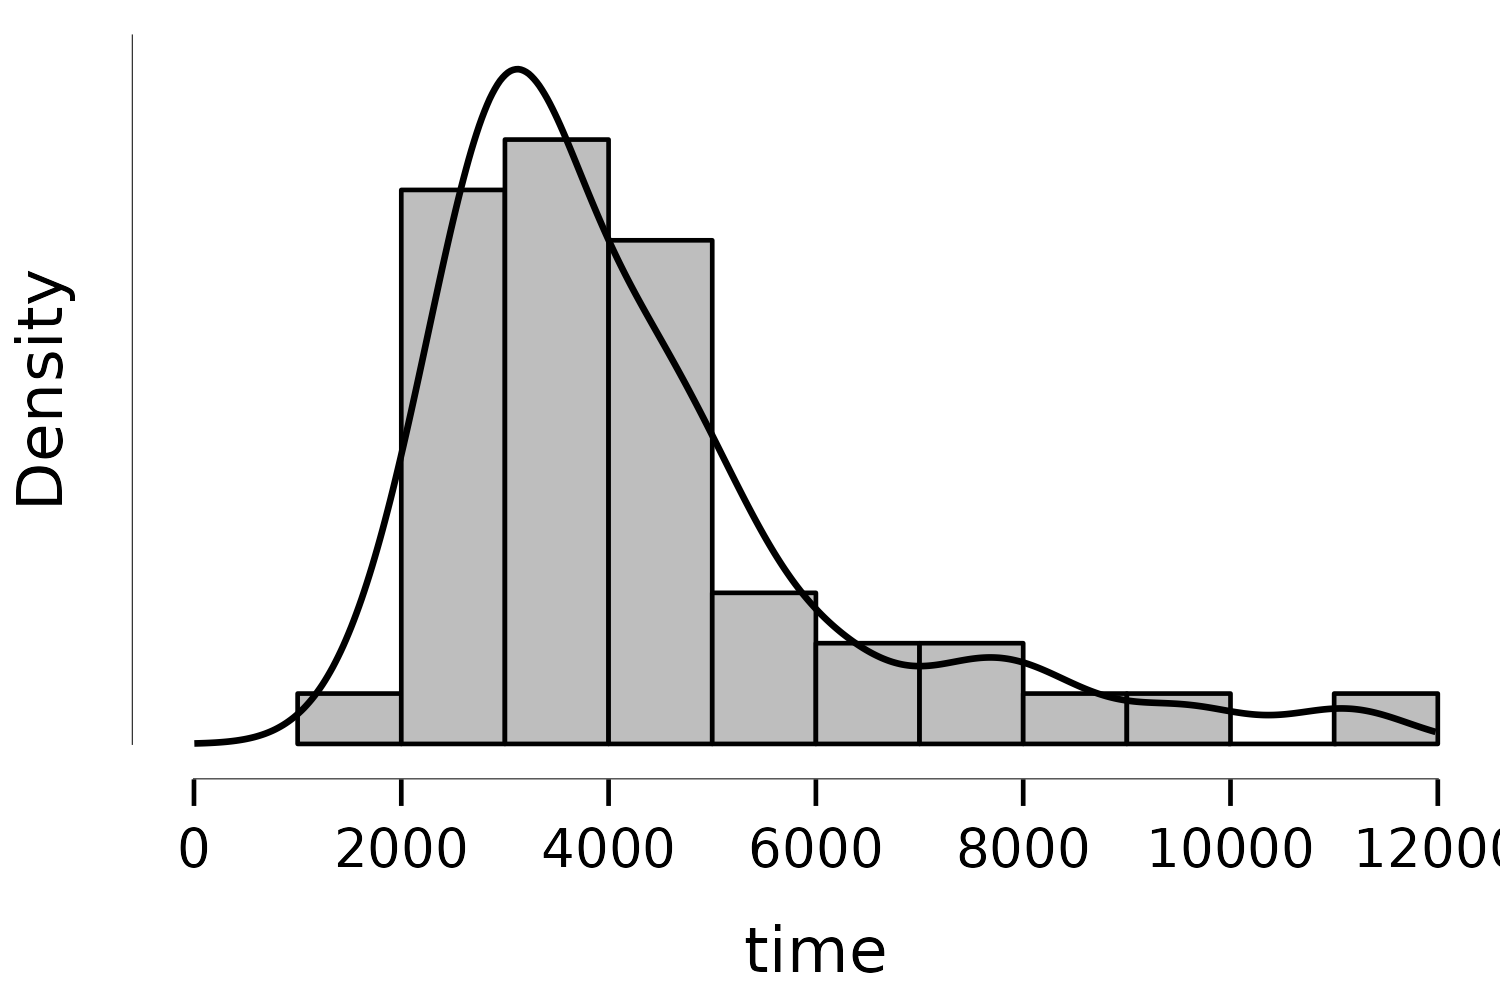
\includegraphics[width=\textwidth]{images/prog_false.png}
			\caption{Distribution of average time for participants without programming knowledge}
		\end{subfigure}
		\begin{subfigure}{0.49\textwidth}
			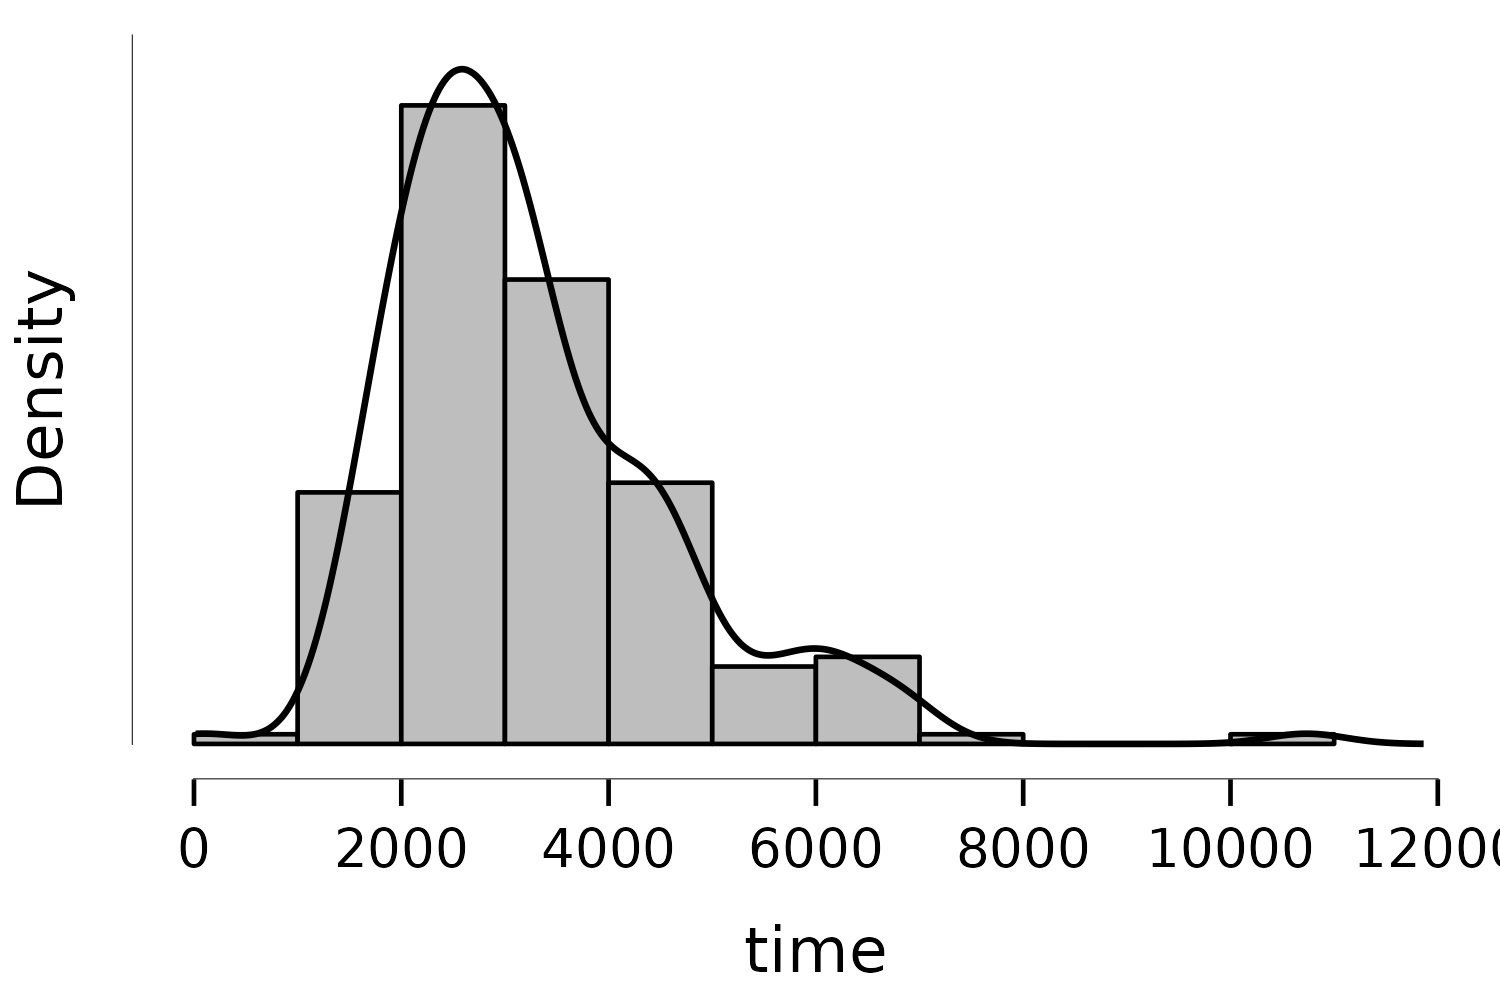
\includegraphics[width=\textwidth]{images/prog_true.png}
			\caption{Distribution of average time for participants with programming knowledge}
		\end{subfigure}
\end{figure}

Given our small population of participants it wasn't possible to draw any meaningful conclusion while looking at the age compared to average
completion time. This is also probably because as said most of the participants had programming knowledge giving less weight to the difference in age.

\subsection{Descriptive Statistics}
We can now look in detail at the specific statistics that we could draw from the experiment. By looking at the table \ref{tab:descriptiveStatistics} we can now 
quantify the difference in performance when using camelCase or kebab-case.

\begin{table}[h]
    \centering
    \caption{Descriptive Statistics}
    \label{tab:descriptiveStatistics}
    {
        \begin{tabular}{lrr}
            \toprule
            \multicolumn{1}{c}{} & \multicolumn{2}{c}{avg. time} \\
            \cline{2-3}
             & camel & kebab  \\
            \cmidrule[0.4pt]{1-3}
            Median & $3805.524$ & $3045.476$  \\
            Mean & $3984.809$ & $3445.125$  \\
            Std. Deviation & $854.439$ & $876.329$  \\
            Minimum & $2688.190$ & $2607.667$  \\
            Maximum & $5349.762$ & $5270.952$  \\
            \bottomrule
        \end{tabular}
    }
\end{table}

While the range of average times registered is pretty much the same, we see some important differences when looking at the mean and especially the median.
We can in fact observe, looking at the median, a $25\%$ improvement in average time in favour of kebab-case as opposed to camelCase. While less prominent there is 
also a $16\%$ increase in perfomance for the mean average time.

\subsection{Inferential Statistics}
To validate our findings we finally make use of inferential statistics, specifically by applying the Students's T-test on the data and then 
calculating the Cohen's d. 

\begin{table}[h]
    \centering
    \caption{Independent Samples T-Test for time depending on separator}
    \label{tab:independentSamplesT-TestSeparator}
    {
        \begin{tabular}{lrrrrr}
            \toprule
            $ $ & t & df & p & Cohen's d & SE Cohen's d  \\
            \cmidrule[0.4pt]{1-6}
            avg. time & $1.462$ & $20$ & $0.080$ & $0.624$ & $0.447$  \\
            \bottomrule
            % \addlinespace[1ex]
            % \multicolumn{6}{p{0.5\linewidth}}{\textit{Note.} For all tests, the alternative hypothesis specifies that group \textit{ camel $<$/em> is greater than group <em> kebab }.} \\
            % \multicolumn{6}{p{0.5\linewidth}}{\textit{Note.} Student's t-test.} \\
        \end{tabular}
    }
\end{table}

\begin{table}[h]
    \centering
    \caption{Independent Samples T-Test for time depending on programming background}
    \label{tab:independentSamplesT-TestProg}
    {
        \begin{tabular}{lrrrrr}
            \toprule
            $ $ & t & df & p & Cohen's d & SE Cohen's d  \\
            \cmidrule[0.4pt]{1-6}
            time & $3.895$ & $229$ & $<$ .001 & $0.653$ & $0.181$  \\
            \bottomrule
            % \addlinespace[1ex]
            % \multicolumn{6}{p{0.5\linewidth}}{\textit{Note.} For all tests, the alternative hypothesis specifies that group \textit{ false $<$/em> is greater than group <em> true }.} \\
            % \multicolumn{6}{p{0.5\linewidth}}{\textit{Note.} Student's t-test.} \\
            % \multicolumn{6}{p{0.5\linewidth}}{$^{0}$ Brown-Forsythe test is significant (p $<$ .05), suggesting a violation of the equal variance assumption} \\
        \end{tabular}
    }
\end{table}

We know that for a result to be accepted the $p$ value should be less than $0.05$ and from table \ref{tab:independentSamplesT-TestSeparator} we can see that while not exactly over the boundary 
we are very close to a significant $p$ value, nonetheless the Cohen's d shows a more than medium effect. From table \ref{tab:independentSamplesT-TestProg} we can instead see a $p$ value significantly 
below the threshold, meaning not only a medium effect but also a valid conclusion that programming experience influences the reading ability of users.


\section{Discussion}

\subsection{Compare Hypothesis to Results}
We deliberately chose to formulate the null hypotheses at the start since we see the choice of the separator mainly as a personal preference. For the same reason 
we wanted to avoid the risk of introducing bias given our subjective experiences.

Contrary to our hypothesis we can actually see some objective differences in reading speed when using camelCase or kebab-case.

\subsection{Limitations and Threats to Validity}
A clear limitation that could (and possibly did) lead to reliable results is the choice of our participant pool. Given the fact that our testing application 
was not put on a server but kept locally (given time constraints and for simplicity) we eneded up asking friends and people around us, who of course eneded up being 
mostly informatics students. Ideally the number of participants should also be increased, in order to get a more fair distribution of age representation and different 
proficiency in coding.

\subsection{Conclusions}
While our research and analysis may not give an advantage backed by statistics to one of the two separators, and we believe that it will remain a choice based on mainly 
preference, we can see significance in doing further research into this topic.

\end{document}
